
In dem Teil wird die komplete innere Logik der Application beschrieben. Dafür ist nur \textbf{Controller} notwendig. 
D.h. beim Geschehen eines Ereignisses wird eine (oder mehrere) Method(en) in deb jeweiligen Controllern aufgerufen,
die das Ereignis entsprechend abarbeiten.
Dabei hat man folgendes Problem:
jeder \textbf{Controller} übernimmt mehrere Aufgaben 
(z.B. Kontrollieren von \textbf{Port} und \textbf{Adapter} und enthält Anwendungslogik)
d.h. keine \textbf{SRP}

Eine mögliche Lösung wäre das Separieren von Kontrollieren von \textbf{Port} und \textbf{Adapter} und Anwendungslogik
in 2 verschiedenen Teile. Die Anwendungslogik heißt \textbf{UseCase}.

Bei dieser Aufteilung besteht das Problem, dass beim Geschehen eines Ereignisses im \textbf{Controller} muss dieses Ereignis an das 
richtige \textbf{UseCase} zugeordnet werden. D.h. \textbf{Contoller} besitzt eine weitere Verantwortlichkeit die sich in ein anderes Teil
verschieben lässt. Dieses Teil heißt \textbf{Dispatcher}, dessen Aufgabe ist das Informieren alle daran Interessierten \textbf{UseCase}s
beim Geschehen eines Ereignisses. 

Jedes \textbf{UseCase} kann mehrere aufeinander folgende Aufgaben machen.
Alle Aufgaben müssen gleiche Funktionalitäten besitzen, z.B:
\begin{itemize}
    \item der Anfang und das Ende in Logs aufzeichnen.
    \item Nach einer bestimmten Zeit gestoppt werden.
\end{itemize}
D.h. man braucht eine ``Hülle'' um jeder Methode - \textbf{Interactor}

Wenn man das alles zusammen entsteht folgendes Objektendiagramm:

\begin{figure}[H]
    \centering
    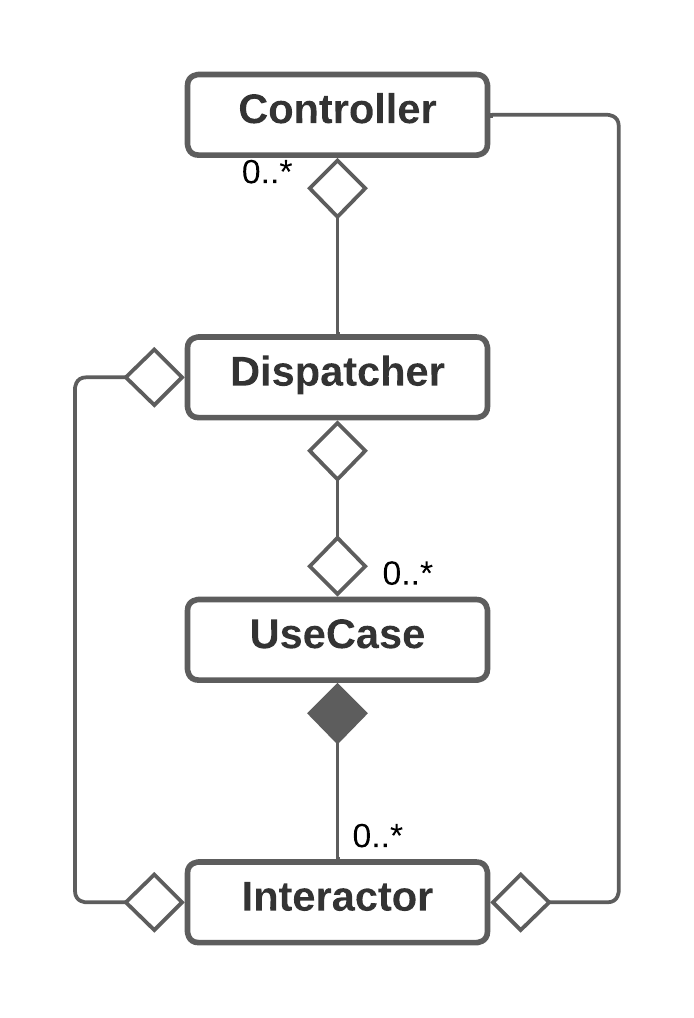
\includegraphics[width=6.5cm]{./images/Controller-Dispatcher-UseCase-Interactor.png}
     \caption[Objektendiagramm Controller-Dispatcher-UseCase-Interactor]{Objektendiagramm Controller-Dispatcher-UseCase-Interactor \footnotemark}
     \label{fig:CDCDUI}
\end{figure}
\footnotetext{Eigene Quelle}
